\section{Detailed Example}
\label{sec:example}

% dzm: this figure might just need to go.
\begin{figure*}
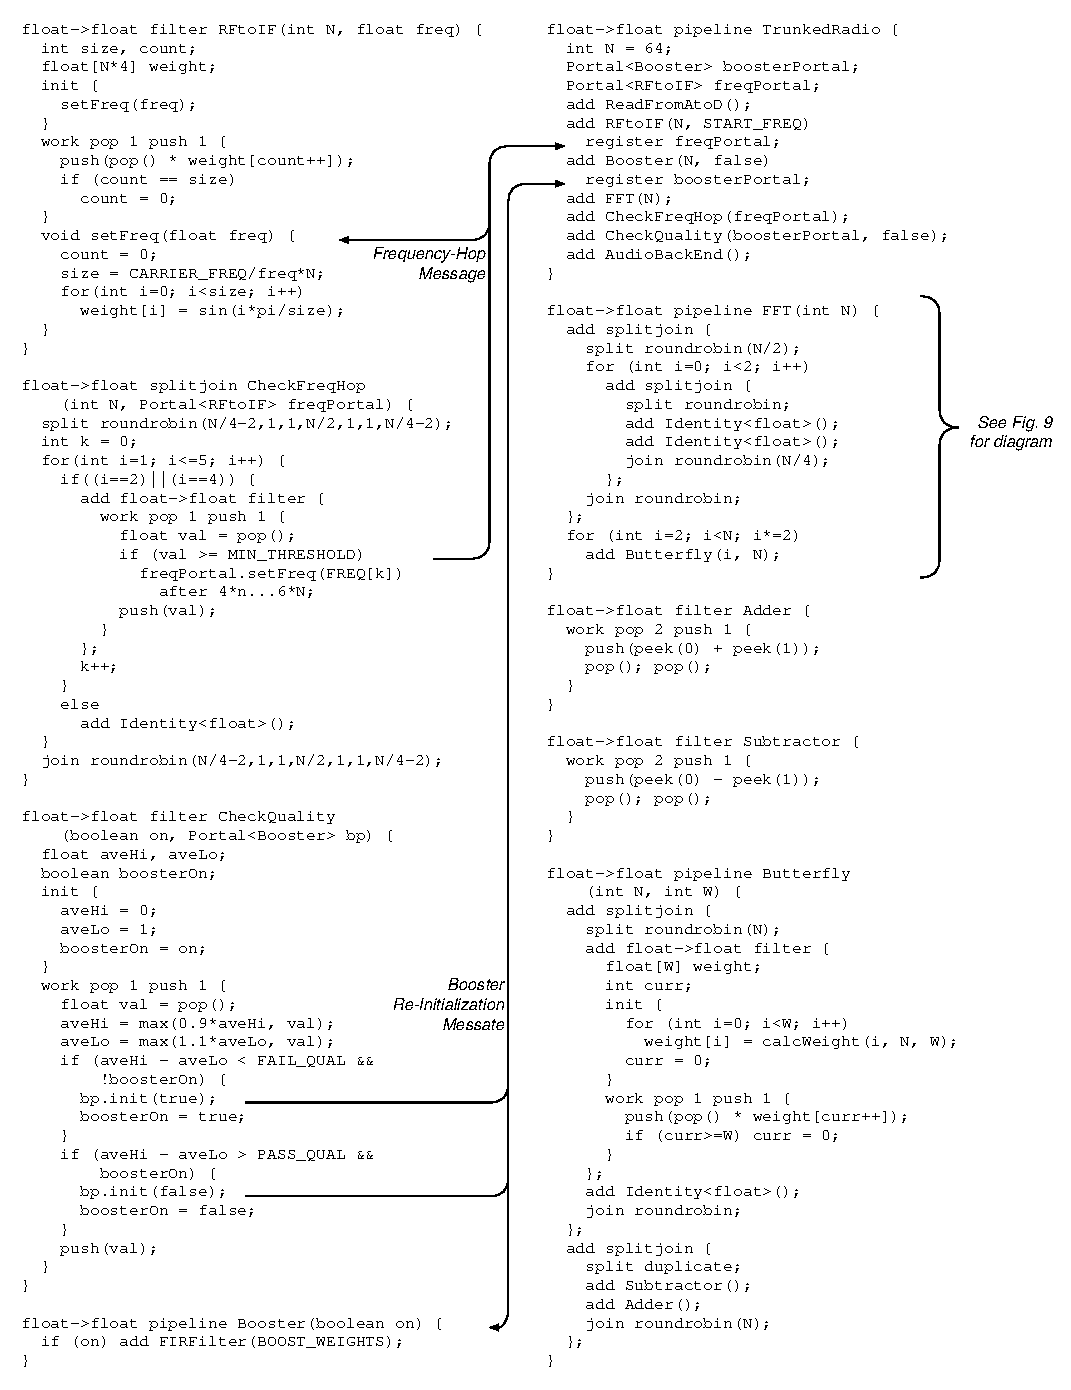
\includegraphics[width=\textwidth]{code-fm.eps}
\caption{StreamIt code for a software radio.  Arrows denote the paths
  of messages.}
\label{fig:radiocode}
\end{figure*}

We now discuss the StreamIt implementation of the Trunked Radio
illustrated in Fig.~\ref{fig:radiodiagram}.  The Trunked Radio is a
frequency-hopping system in which the receiver switches between a set of
known frequencies whenever it hears certain tones from the transmitter.

The toplevel class, \texttt{TrunkedRadio}, is implemented as a
seven-stage pipeline (see Fig.~\ref{fig:radiocode}).  The
\texttt{RFtoIF} stage modulates the input signal from RF to a
frequency band around the current IF frequency.  To support a change
in the IF frequency when frequency hopping occurs, the \texttt{RFtoIF}
filter contains a \texttt{setFreq} method that is invoked via a
message from the \texttt{CheckFreqHop} stage.  The message is sent
from \texttt{CheckFreqHop} with a latency range of $4N$ to $6N$, which
means that \texttt{RFtoIF} must deliver between $4N$ and $6N$ items
using the old modulation scheme before changing to the new frequency.

The optional \texttt{Booster} stage provides amplification for weak
signals, but is usually turned off to conserve power.  The
\texttt{Booster} is toggled by a re-initialization message from the
\texttt{CheckQuality} stage, which estimates the signal quality by the
shape of the frequency spectrum.  If all the frequencies have similar
amplitudes, \texttt{CheckQuality} assumes that the signal-to-noise
ratio is low and sends a message to activate the \texttt{Booster}.
This message is sent using best-effort delivery.

The \texttt{FFT} stage converts the signal from the time domain to the
frequency domain; please refer to p.~796 of \cite{clr} for a diagram
of the parallel FFT algorithm.  The StreamIt implementation consists
of a bit-reversal permutation followed by a series of
\texttt{Butterfly} stages.  The bit-reversal phase illustrates how
data can be reshuffled with just a few SplitJoin constructs (see
Fig.~\ref{fig:bitreverseorder}).  The \texttt{Butterfly}
stage--which is parameterized to allow for a compact representation of
the FFT--also employs split-joins to select groups of items for its
computation.  We believe that the StreamIt version of the FFT is clean
and intuitive, as the SplitJoin constructs expose the natural
parallelism of the algorithm.

%%% Local variables:
%%% TeX-master: "paper.tex"
%%% End:
